\subsection{Identifizierung der ben�tigten Modelle}
Modelle tauchen in Abbildung~\ref{fig:guiClass} nicht auf, da das GUI-Framework kein Interface und keine Zugriffswege f�r Modelle vorgibt. Dies erm�glicht einem \emph{Presenter}-\emph{View}-Paar die Verwendung mehrere Modelle, wovon die Implementierung des \DevEnvs\ auch Gebrauch macht. Insgesamt werden zur Umsetzung der Systemanforderungen sechs Modelle ben�tigt, die im Designmodell mit dem Stereotyp \texttt{model} gekennzeichnet sind.

\begin{itemize}
	\item \texttt{\textbf{Horde3DApplication}}: Die \texttt{Horde3DApplication}-Klasse repr�sentiert die \Horde-An-wendung, in der gerade der Server l�uft oder die gestartet werden kann. Sie ist die einzige Zugriffsm�glichkeit auf Operationen des Servers.
	
	\item \texttt{\textbf{CallbackHandler}}: Der \texttt{CallbackHandler} nimmt die \emph{Callbacks} des Servers entgegen und generiert f�r jede Nachricht ein entsprechendes \emph{Event}. Die \emph{Presenter} k�nnen sich an der \texttt{CallbackHandler}-Instanz an verschiedenen Ereignissen registrieren, um �ber Server-Nachrichten informiert zu werden.
	
	\item \texttt{\textbf{MessagesDispatcher}}: Die Aufgabe des \texttt{MessagesDispatcher}-Modells ist die Verwaltung aller erzeugten Nachrichten. Die Nachrichten k�nnen zum einen aus der \Horde-Anwendung stammen oder vom Client generierte Fehler- oder Debugmeldungen sein. Die Nachrichten werden nach ihrer Herkunft (Client oder Server) kategorisiert und nach Wichtigkeit (Debug, Information, Warnung oder Fehler) unterschieden. Der \emph{Dispatcher} unterst�tzt auch das Entfernen aller Nachrichten einer bestimmten Kategorie. Nachdem Meldungen entfernt oder hinzugef�gt wurden, wird ein spezielles Ereignis ausgel�st, damit die interessierten \emph{Presenter} und \emph{Views} entsprechend reagieren k�nnen.
	
	\item \texttt{\textbf{SceneGraph}} und \texttt{\textbf{ResourceGraph}}: Diese beiden Modelle dienen zum Verwalten aller bekannten \emph{Scene Nodes} und Ressourcen. Werden neue Objekte eingef�gt oder Objekte entfernt, wird ein \texttt{GraphChanged}-\emph{Event} ausgel�st, um die �nderungen bekannt zu machen.
	
	\item \texttt{\textbf{ProfilingDataManager}}: Dieses Modell funktioniert �hnlich der beiden zuvor genannten Modelle und verwaltet die Profiling-Daten. Das \texttt{ProfilingDataChanged}-\emph{Event} wird ausgel�st, wenn Profiling-Daten empfangen oder gel�scht werden.
\end{itemize}

\begin{figure}[htp]
\centering
%trim=l b r t  	This option will crop the imported image by l from the left, b from the bottom, r from the right, and t  from the top. Where l, b, r and t are lengths. 
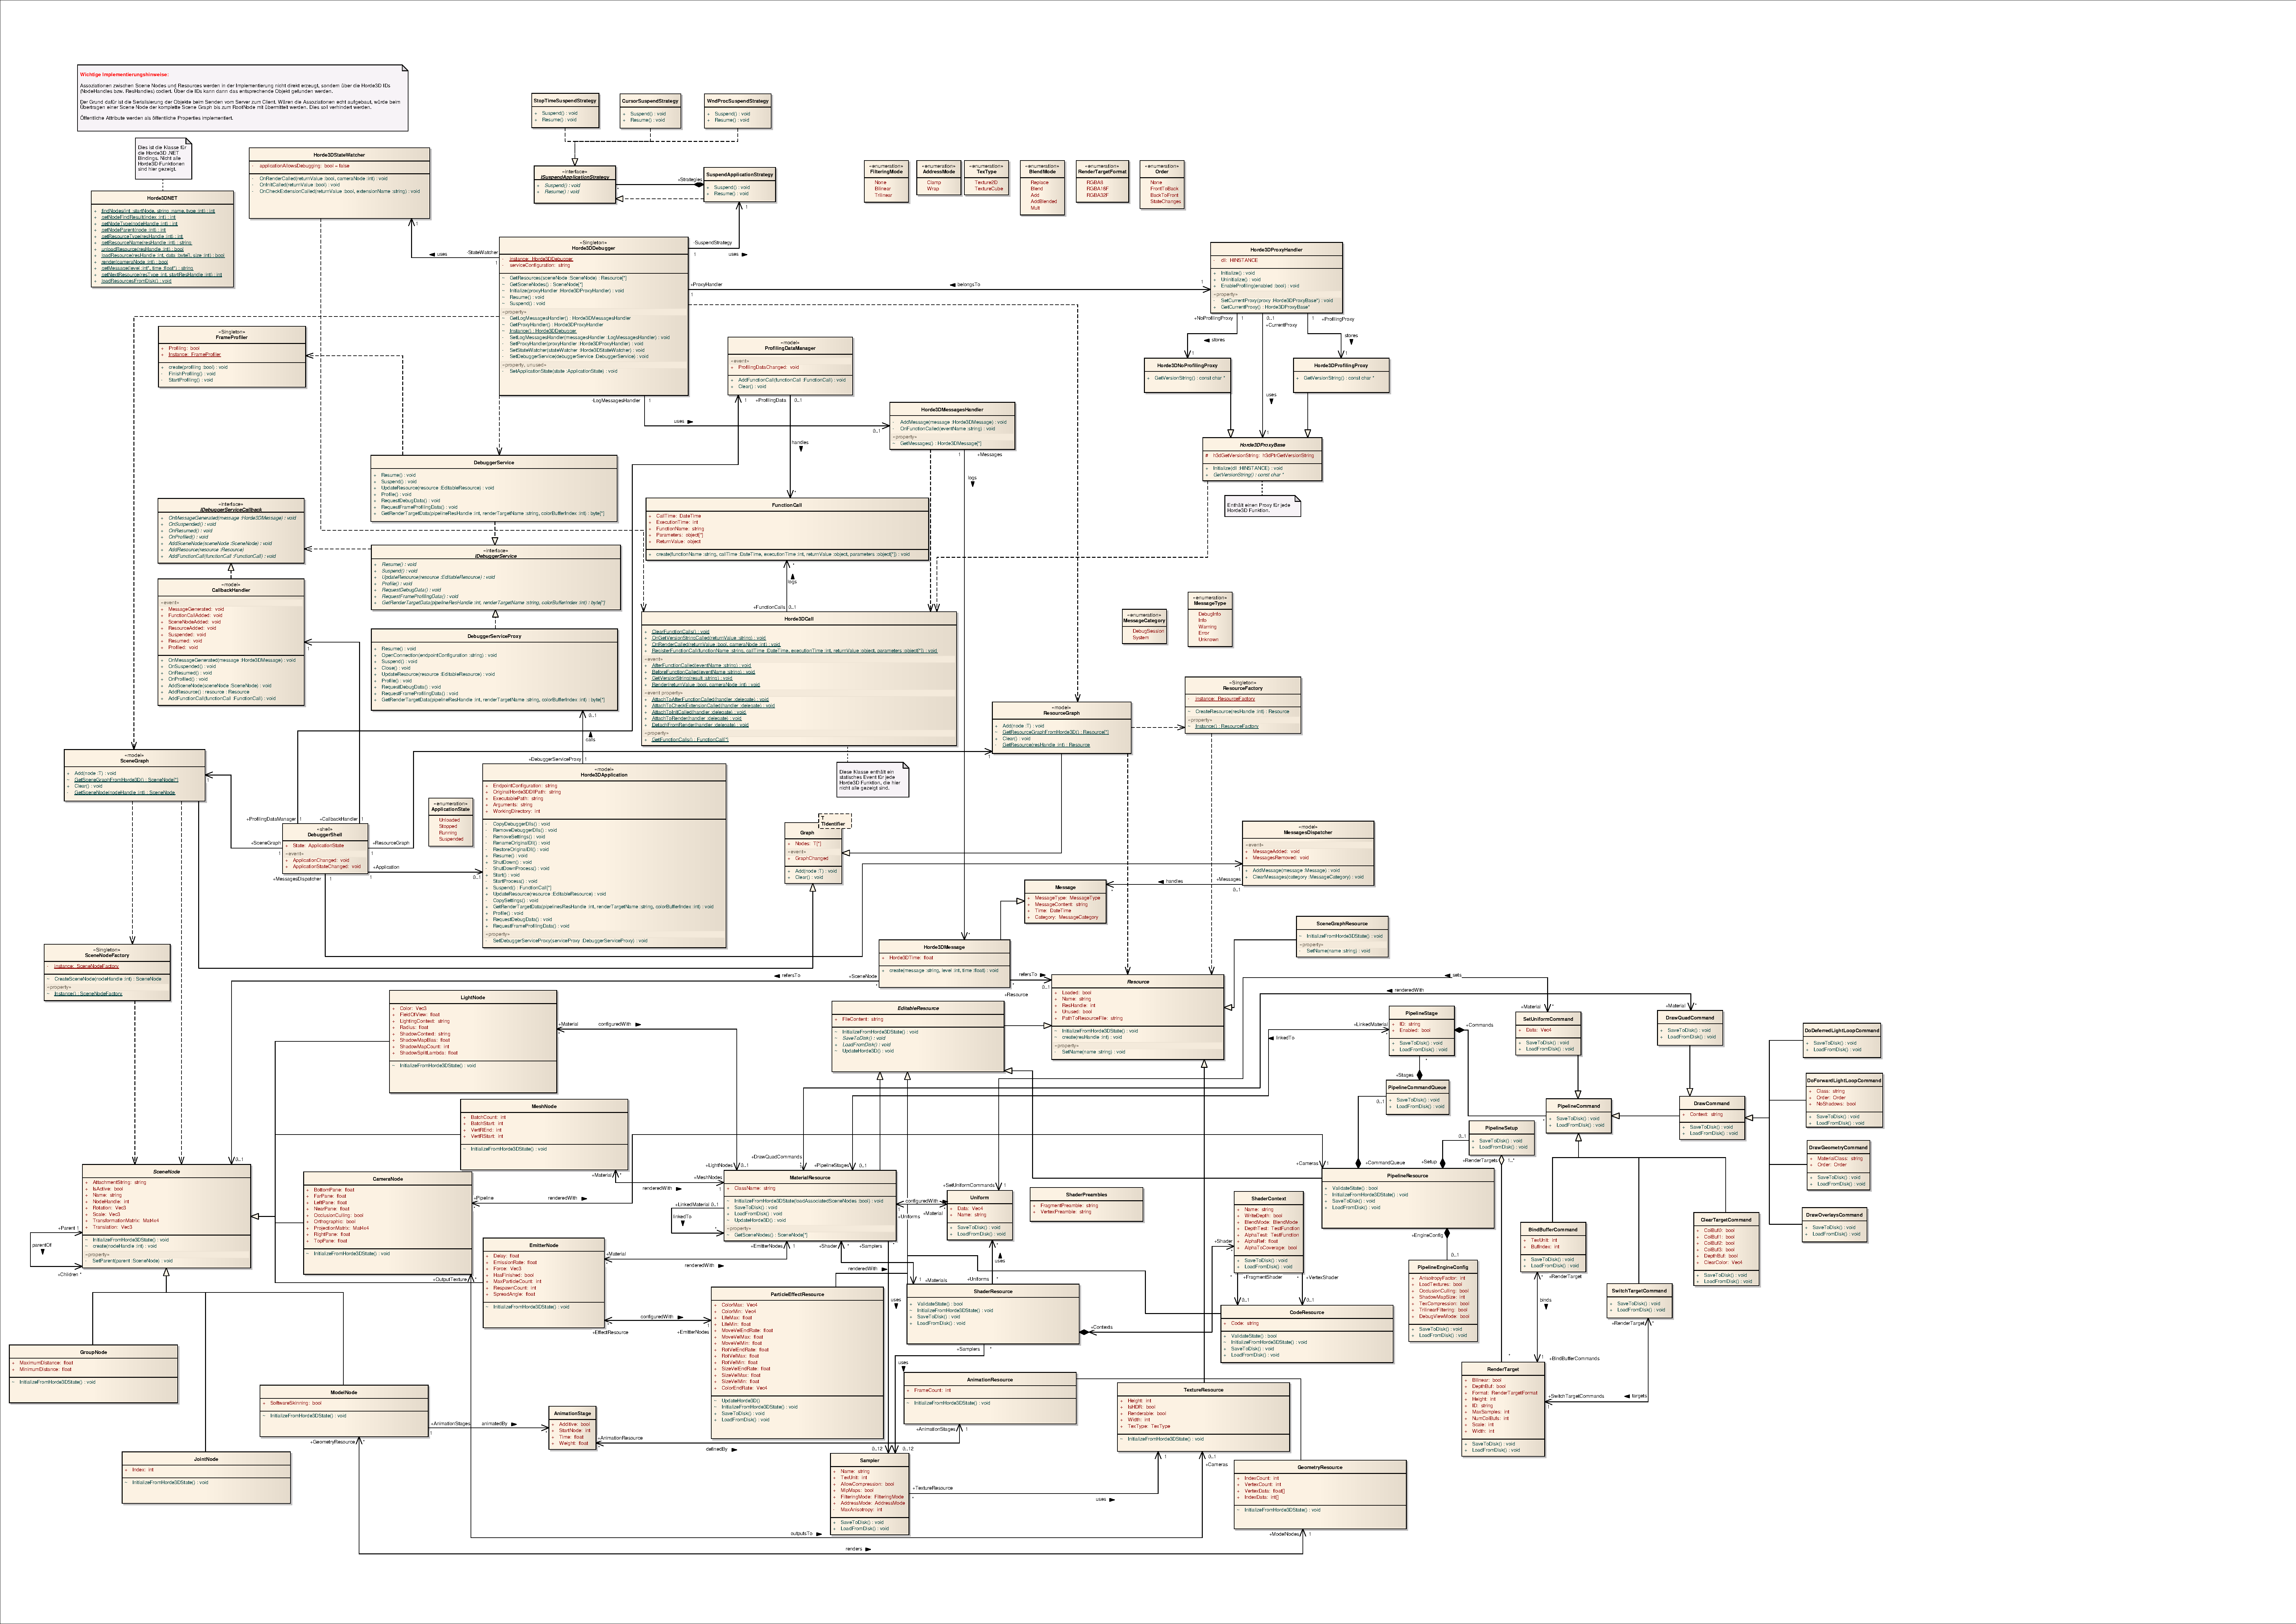
\includegraphics[trim = 125mm 380mm 975mm 415mm, clip, scale=0.7]{images/Designmodell.pdf}
\caption{Die Shell des \DevEnvs\ im Designmodell}\label{fig:shellDesign}
\end{figure}

Alle Modelle werden von der \texttt{Shell}-Klasse verwaltet, wodurch alle \emph{Presenter} Zugriff auf alle Modelle erhalten. Die \texttt{Shell}-Klasse �berwacht au�erdem den aktuellen Zustand des Servers, da einige \emph{Presenter} und \emph{Views} bei Zustands�nderungen spezielle Aktionen durchf�hren m�ssen. Die m�glichen Zust�nde sind \texttt{Unloaded}, wenn derzeit kein \texttt{Horde3DApplication}-Modell geladen ist und somit der Server nicht gestartet werden kann; \texttt{Stopped}, wenn der Server zur Zeit nicht l�uft aber gestartet werden kann; \texttt{Suspended}, wenn der Server gerade l�uft und die Szene eingefroren ist; und \texttt{Running} sonst. Die \texttt{Shell}-Klasse l�st ein \emph{Event} aus, sobald sich der Zustand des Servers �ndert.